\documentclass{article}
\usepackage[a4paper,left=3cm,right=3cm,top=1cm,bottom=2cm]{geometry}
\usepackage{amsmath}
\usepackage{amssymb}
\usepackage{hyperref}

\usepackage{tikz-cd}
\usepackage{adjustbox}
\usepackage{wrapfig}
\usepackage{tkz-euclide}
\setlength{\parindent}{0mm}

\usepackage{fontspec}
\setmainfont{Linux Libertine O}
\usepackage{unicode-math}
\setmathfont{Cambria Math}

\title{
\textit{\small{Георгий Потошин, 2024}}\\
\vspace{0.3ex}
\textit{\huge{Топология I, листочек 4}}\vspace{1ex}
}

\date{\vspace{-10ex}}

\begin{document}
\maketitle
\textit{Я буду здесь и далее обозначать открытость конца интервала через
    квадратную скобку, смотрящую наружу. То есть интервал между 0 и 1 будет
    записываться как $]0,1[$.}

\begin{enumerate}
    \item 
        \textbf{Что получится, если разрезать ленту Мёбиуса по средней линии?
        А если повторить процедуру?}

        Лента Мёбиуса определятся как фактор пространство квадрата $I^2/\sim$,
        где $I=[0,1]$, а отношение эквивалентности объединяет в один класс
        точки $(a,0)$ и $(1,1-a)$. Выкинем из ленты отрезок между точками
        $(0,0.5)$ и $(1,0.5)$. Полученное пространство будет линейно связным.
        назавем $H_+=[0,1]\times]0.5,1]$ верхнюю часть и $H_-=[0,1]\times
        [0,0.5]$. Заметим, что факторизация не связывает точки $H_+$ между
        собой, а значит $H_+$ гомеоморфно квадрату без одной стороны, а он
        линейно связен. Тоже самое можно сказать и про $H_-$. Тогда пусть $A\in
        H_-$ и $B\in H_+$. Тогда точку $A$ можно связать прямой с точкой $M=
        (0,0)$, которая по факторизации эквивалентна точке $N=(1,1)$, a уже её
        можно связать с точкой $B$. Тогда отображение $(t\in[0,0.5]\mapsto A+2t
        \overrightarrow{AM})\cup(t\in[0.5,1]\mapsto N + (2t-1)\overrightarrow{NB})$
        опишет путь из $A$ в $B$ и будет непрерывным. А значит разрезанная
        лента Мёбиуса линейно связна.

        \begin{center}
        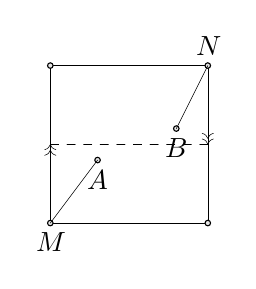
\begin{tikzpicture}[scale=1]
            \tkzDefPoints{0/0/M, 0/2/P, 2/2/N, 2/0/Q, 0.6/0.8/A, 1.6/1.2/B,
                          0/1/S, 2/1/T}
            \begin{scope}[decoration={
                markings,
                mark=at position 0.5 with {\arrow{>>}}}]
            \tkzDrawSegment[postaction={decorate}](M,P)
            \end{scope}
            \tkzDrawSegment(P,N)
            \begin{scope}[decoration={
                markings,
                mark=at position 0.5 with {\arrow{>>}}}]
            \tkzDrawSegment[postaction={decorate}](N,Q)
            \end{scope}
            \tkzDrawSegment(Q,M)
            \tkzDrawSegment[dashed](S,T)
            \tkzDrawPoints(M,P,N,Q,A,B)
            \tkzDrawSegment(A,M)
            \tkzDrawSegment(B,N)
            \tkzLabelPoints(M,A,B)
            \tkzLabelPoints[above](N)
        \end{tikzpicture}
        \end{center}

        Теперь повторим процедуру, вырезав ещё отрезки $[0,1]\times\{0.75\}$ и
        $[0,1]\times\{0.25\}$. Тогда нетрудно видеть, что лента распадется на
        2 несвязные части.

        \begin{center}
        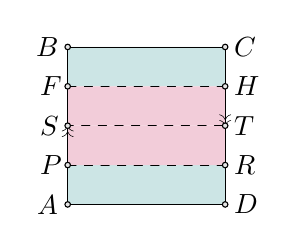
\begin{tikzpicture}[scale=1]
            \tkzDefPoints{0/0/A, 0/2/B, 2/2/C, 2/0/D, 0/1/S, 2/1/T, 0/0.5/P,
            2/0.5/R, 0/1.5/F, 2/1.5/H}
            \tkzDrawPolygon[fill=teal!20,dashed](F,H,C,B)
            \tkzDrawPolygon[fill=teal!20,dashed](P,R,D,A)
            \tkzDrawPolygon[fill=purple!20,dashed](F,H,T,S)
            \tkzDrawPolygon[fill=purple!20,dashed](P,R,T,S)
            \begin{scope}[decoration={
                markings,
                mark=at position 0.5 with {\arrow{>>}}}]
            \tkzDrawSegment[postaction={decorate}](A,B)
            \end{scope}
            \tkzDrawSegment(B,C)
            \begin{scope}[decoration={
                markings,
                mark=at position 0.5 with {\arrow{>>}}}]
            \tkzDrawSegment[postaction={decorate}](C,D)
            \end{scope}
            \tkzDrawSegment(D,A)
            \tkzDrawPoints(A,B,C,D,S,T,P,R,F,H)
            \tkzLabelPoints[right](C,H,R,T,D)
            \tkzLabelPoints[left](A,P,S,F,B)
        \end{tikzpicture}
        \end{center}

        Это верно из того соображения, что если склеить красные кусочки через
        $ST$ и синие через $FH$ и $PR$, то выйдут 2 ленты Мёбиуса, а их
        разрезание по месту склейки оставит их связными.

    \item
        \textbf{Докажите, что следующие определения $\mathbb{R}P^n$ эквивалентны:\vspace{1ex}\\
                $(i)$ сфера в $\mathbb{R}^{n+1}$ с отождествленными
                противоположными точками;\vspace{1ex}\\
                $(ii)$ диск $D^n$ с отождествленными противоположными
                точками границы $\partial D^n = S^{n−1}$;\vspace{1ex}\\
                $(iii)$ множество всех прямых в $\mathbb{R}^{n+1}$, проходящих
                через начало координат (введите на этом множестве естественную
                топологию);\vspace{1ex}\\
                $(iv)$ множество всех гиперплоскостей в $\mathbb{R}^{n+1}$,
                проходящих через начало координат (введите на этом множестве
                естественную топологию).}
                
        $(i)\simeq(ii)$ Диск можно непрерывно вложить в сферу следующим образом.
        \[\varphi:(x_1,...,x_n)\mapsto(\sqrt{1-x_1^2-...-x_n^2},x_1,...,x_n)\]
        Пусть факторизация диска и сферы из условия заданны соответственно
        отображениями $\pi_D$ и $\pi_S$. Дополним диаграмму с $\varphi$
        отображением $\varphi'$ естественным образом, чтобы она коммутировала.

        \begin{center}
        \begin{tikzcd}
            D^n\arrow{r}{\varphi} \arrow[swap]{d}{\pi_D} & S^n \arrow{d}{\pi_S} \\
            D^n/\!\sim \arrow{r}{\varphi'} & S^n/\!\sim
        \end{tikzcd}
        \end{center}

        Это возможно в силу того, что $\varphi$ переводит элементы одного
        класса в один и тот же класс. $\varphi'$ – очевидно биекция. $\varphi$
        – непрерывное отображение, причем очевидно, что оно является
        непрерывной биекцией из компактного диска в хаусдорфову полусферу, а
        значит $\varphi$ переводит отрытые в открытые. Отображение $\pi_S$ и
        $\pi_D$ являются непрерывными. К тому же $\pi_S$ переводит открытые в
        открыты, так как $\pi_S^{-1}[\pi_S[U]] = U \cup -U$ – открыто,
        отображение $\pi_D$ переводит в открытые множества, открытые и симметричные по
        границе $-\partial D^n\cap U=\partial D^n\cap U$ относительно центра.
        Тогда $\varphi'[U]=\pi_S[\varphi[\pi_D^{-1}[U]]]$ переводит открытые в
        открытые, точно также прообразы открытых открыты $\varphi'^{-1}[V]=
        \pi_D[\varphi^{-1}[\pi_S^{-1}[V]]]$, аргумент $\pi_D$ здесь симметричен
        по границе относительно центра. Тогда $\varphi'$ – гомеоморфизм и
        $D^n/\!\sim\,\simeq S^n/\!\sim$.

        $(i) \sim (ii)$ Здесь прямые можно отождествить с их пересечениями на
        сфере, а расстояние между прямыми задать как угол между ними, что тоже
        самое, что длина минимальной из 2 дуг соединяющих точки пересечения.
        Пусть $L$ – множество прямый, а $S$ – сфера. Тогда будут две проекции
        $\pi_L: S \longrightarrow L$, ставящая точке прямую через неё проходящую,
        и $\pi_S: S \longrightarrow S/\!\sim$. Тогда можно будет дополнить диаграмму:

        \begin{center}
        \begin{tikzcd}[column sep=small]
            & S \arrow[dl, swap, "\pi_L"] \arrow[dr, "\pi_S"] &   \\
            L \arrow[rr, "\varphi"] & & S/\!\sim
        \end{tikzcd}
        \end{center}

        Потому как обе проекции делят шар на одинаковые классы. Прообразами
        шаров при $\pi_L$ будут двойные шары $B \cup -B$, а они
        открыты. Образом же шара из $S$ будет пучок прямы, проходящий через этот
        шар и центр сферы, а он открыт. Тогда $\pi_L$ переводит открытые в
        открытые, а также непрерывно. Тогда как и в прошлом пункте если
        проходить между $L$ и $S/\!\sim$ через $S$, то открытые будут оставаться
        открытыми.

        $(iii)\simeq(iv)$ Здесь стоит заметить, что углы между плоскостями и
        прямыми, перпендикулярными к ним совпадают, а значит сопоставляя
        плоскости её ортогональное дополнение, мы построим биективную изометрию,
        а значит и гомеоморфизм.

    \item \textbf{Докажите, что следующие пространства попарно гомеоморфны
        (по определению, все они называются комплексным проективным
        пространством $\mathbb{C}P^n$):\\
        (i) сфера $S^{2n+1}$ в $\mathbb{C}^{n+1} = \mathbb{R}^{2n+2}$ с
        отождествленными точками вида $x\sim\lambda x$ для $\lambda\in\mathbb{C}
        , |\lambda| = 1$;\\
        (ii) диск $D^{2n}\in\mathbb{C}^n = \mathbb{R}^{2n}$ с отождествленными
        противоположными точками границы $\partial D^{2n} = S^{2n−1}$
        вида $x\sim\lambda x$ для $\lambda\in\mathbb{C}$, $|\lambda|=1$;\\
        (iii) множество всех комплексных прямых $\mathbb{C}$ в
        $\mathbb{C}^{n+1}$, проходящих через начало координат (введите на этом
        множестве естественную топологию);\\
        (iv) множество всех комплексных гиперплоскостей $\mathbb{C}^n$ в
        $\mathbb{C}^{n+1}$, проходящих через начало координат (введите на этом
        множестве естественную топологию).}

        \textit{Я буду использовать далее следующее обозначение $\mathbb{U}=
        \{z\in\mathbb{C}\;|\;|z|=1\}.$}

        $(i)\simeq(ii)$ Здесь доказательство такое же, как и в действительном
        случае, кроме того, что отображение $\varphi$ задается иначе.
        \[\varphi:(x_1,...,x_n)\mapsto(\sqrt{1-x_1\overline{x_1}-...-x_n
        \overline{x_n}},x_1,...,x_n)\]
        Также достроим диаграмму:

        \begin{center}
        \begin{tikzcd}
            D^n\arrow{r}{\varphi} \arrow[swap]{d}{\pi_D} & S^n \arrow{d}{\pi_S} \\
            D^n/\!\sim \arrow{r}{\varphi'} & S^n/\!\sim
        \end{tikzcd}
        \end{center}

        Это возможно в силу того, что $\varphi$ переводит элементы одного
        класса в один и тот же класс. $\varphi'$ – очевидно биекция. $\varphi$
        – непрерывное отображение, причем очевидно, что оно является
        непрерывной биекцией из компактного диска в хаусдорфову полусферу, а
        значит $\varphi$ переводит отрытые в открытые. Отображение $\pi_S$ и
        $\pi_D$ являются непрерывными. К тому же $\pi_S$ переводит
        открытые в открыты, так как $\pi_S^{-1}[\pi_S[U]] = \mathbb{U}U$ –
        объединение отрытых – открыто, отображение $\pi_D$ переводит в открытые
        множества, симметричные по границе $\mathbb{U}(\partial D\cap U)=\partial
        D\cap U$ относительно центра. Тогда
        $\varphi'[U]=\pi_S[\varphi[\pi_D^{-1}[U]]]$ переводит открытые в
        открытые, точно также прообразы открытых открыты $\varphi'^{-1}[V]=
        \pi_D[\varphi^{-1}[\pi_S^{-1}[V]]]$, аргумент $\pi_D$ здесь симметричен
        по границе относительно центра. Тогда $\varphi'$ – гомеоморфизм и
        $D^n/\!\sim\,\simeq S^n/\!\sim$.

        $(i) \sim (ii)$ Здесь прямые можно отождествить с их пересечениями на
        сфере, а расстояние между прямыми задать как минимальное расстояние
        между унитарными векторами этих прямых. Пусть $L$ – множество прямый, а
        $S$ – сфера. Тогда будут две проекции $\pi_L: S \longrightarrow L$,
        ставящая точке прямую через неё проходящую, и $\pi_S: S \longrightarrow 
        S/\!\sim$. Тогда можно будет дополнить диаграмму:

        \begin{center}
        \begin{tikzcd}[column sep=small]
            & S \arrow[dl, swap, "\pi_L"] \arrow[dr, "\pi_S"] &   \\
            L \arrow[rr, "\varphi"] & & S/\!\sim
        \end{tikzcd}
        \end{center}

        Потому как обе проекции делят шар на одинаковые классы. Непрерывная
        проекция $\pi_S$, как мы видели ранее переводит открытые в открытые.
        Покажем, что проекция $\pi_L$ действует также. Пусть $B^r_L=\{a\;|\;
        d(a,c)<r\}$ – шар прямых, расстояние которых до выделенной прямой $c$
        меньше $r$. Пусть $S=\pi_L^{-1}[B^r_L]$ и $C=\pi_L^{-1}(c)$ очевидно,
        что прямая однозначно определяется унитарным вектором, лежащим в ней и
        пусть $e\in C$ – унитарный вектор центральной прямой. Тогда для $x\in S$
        будет верно следующее $\|\lambda a - \mu e\|<r$ для некоторых $\lambda,
        \mu\in\mathbb{U}$, на самом деле внутри нормы можно сократить на
        унитарную $\lambda$ и останется $\|a -\mu e\|<r$ для другого $\mu$.
        Это соотношение будет определяющим для $S$ и мы получим
        $S=\mathbb{U}B^r_e$, а значит $S$ – открыто, а $\pi_L$ – непрерывно.
        В обратную сторону, нетрудно видеть, что $\pi_L^{-1}[\pi_L[B^r_e]]=
        \mathbb{U}B^r_e=\pi_L^{-1}[B^r_c]$ и так как $\pi_L$ – сюръекция, то
        $\pi_L[B^r_e]=B^r_c$. Тогда образ открытого под действием $\pi_L$
        открыт. А тогда точно также как и вдействительном случае, $\varphi$
        сопосталяет открытым открытые в обе стороны.

        $(iii)\sim(iv)$ Здесь также строим изометрию как и в действительном
        случае.

    \item \textbf{Докажите, что $S^n ∗ S^m = S^{n+m+1}$}

        Пусть $(a_1,\ldots,a_n)\in S^n$ и $(a_{n+1},...,a_{n+m})\in S^m$. Сферы
        мы будем считать круглыми, то есть суммы квадратов их координат равны 1.
        Попробуем найти нормировочный член $t\in[-1,1]$ и $n_t^2(\sum a_i^2)+
        t^2=1$, то есть $n_t = \sqrt{(1-t^2)/2}$. Тогда мы сможем отправить
        произведе

        \[\varphi: [((a_1,...,a_n), (b_1,...,b_m), t)]\mapsto (n_ta_1,...,n_tb_1,
        ..., t)\]

        не трудно видеть, что он склеивает точки при $t=\pm 1$. Тогда можно
        дополнить диаграмму:

        \begin{center}
        \begin{tikzcd}
            S^n\times S^m\times I\arrow[r, "\varphi"] \arrow[d, swap, "\pi"] & S^{n+m+1} \\
            S^n*S^m \arrow[ur,swap,"\varphi'"] &
        \end{tikzcd}
        \end{center}

        Очевидно, что $\varphi'$ – биекция. Проверим её непрерывность в обе
        стороны. $\pi$ и $\varphi$ – непрерывны. Пусть $U\subseteq S^n*S^m$ –
        открыт, тогда $\pi^{-1}[U]$ тоже открыто, если в $\pi^{-1}[U]$ нет
        точек, с последней координатой $\pm1$, то так как ограничение $\varphi$
        на произведения, где вместо отрезка взят интервал очевидно является
        непрерывной биекцией, и более того в обратную сторону она тоже непрерывна:
        $(a_1/n_t,...,a_{n+m}/n_t,t)$, то $\varphi'[U]=\varphi[\pi^{-1}[U]]$ –
        открыто. Если всё же $\pi^{-1}[U]$ содержит точки с последней
        координатой $\pm1$, то тогда она содержит все точки с соответствующим
        $\pm1$, назовем множества точек у которых последняя координата равна
        $1$(соответственно $-1$) $P_+$(соответственно $P_-$). Так как
        $\pi^{-1}[U]$ – открыто в регулярном пространстве, то оно содержит слой
        $S^n\times S^m\times]1-\delta,1]$
        вокруг $P_+$ или $P_-$ 

\end{enumerate}
\end{document}
